\newpage
\chapter*{Introduction}
\addcontentsline{toc}{chapter}{Introduction}

"Over the years \gls{Arduino} has been the brain of thousands of projects, from everyday objects to complex scientific instruments. A worldwide community of makers - students, hobbyists, artists, programmers, and professionals - has gathered around this open-source platform, their contributions have added up to an incredible amount of accessible knowledge that can be of great help to novices and experts alike."~\citep{arduino-15-a} 

%
\begin{figure}[ht]
	\centering
	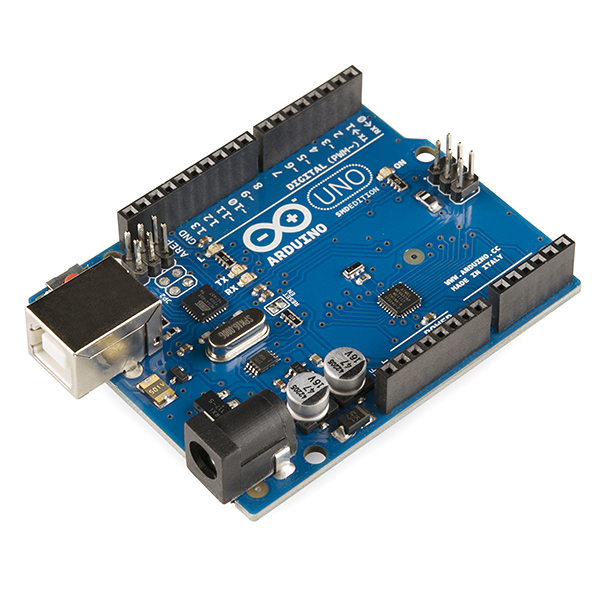
\includegraphics[width=8cm]{images/01}
	\caption{Arduino Uno R3 \citep{wikipedia-13}}
	\label{fig:arduino_uno_r3}
\end{figure}
%

\section*{Where might an Arduino be used?}
\addcontentsline{toc}{section}{Where might an Arduino be used?}
A few contrived examples of where one might use an Arduino in order to automate some process:

\subsection*{Automatic Dog's Water Bowl}
An dog owner wants to ensure her pet is never left without water. She attaches a system for measuring the water level in the dog's bowl. Her \gls{Arduino} is programmed to measure this value every 5 minutes. If this level falls below a certain value, a valve is opened and a water pump is activated to fill up the water bowl. It then sends an SMS to the owner to let her know that the dog is in safe hands.

\begin{itemize}
	\item Read inputs from a water level sensor
	\item Control a valve which lets water flow
	\item Control speed of a water pump 
	\item Send SMS to owner about giving the dog water
\end{itemize}


\subsection*{Bird Table Camera}
A rising social media ornithologist wishes to share pictures from all the visitors to the bird table in his garden. He mounts an infra-red movement sensor on the bird table attached to an \gls{Arduino} which is configured to record an image and send it to Twitter. His neighbours marvel at how many crows he's feeding.

\begin{itemize}
	\item Read inputs from a movement sensor
	\item Control a camera shutter
	\item Transmit image back to PC
	\item Send tweet with picture of the bird table visitor
\end{itemize}


\subsection*{Fingerprint Door Lock}
A student is sick of forgetting his keys and being locked out of his house. He uses a fingerprint scanner and an Arduino to make a biometric fingerprint door lock. He needs only scan his thumb print now and the door will unlock.

\begin{itemize}
	\item Read inputs from a fingerprint sensor
	\item Compares the finger print against an authorised fingerprint
	\item Records the time and date a finger was pressed on the scanner
	\item Makes audio error tone if the fingerprint was invalid
	\item If valid fingerprint it unlocks the door
\end{itemize}


\newpage
\section*{Workshop Aims}
\addcontentsline{toc}{section}{Workshop Aims}
In this workshop the aim is to give you a crash course in digital electronics, and providing you the basic skills to start using the Arduino micro-controllers in your future projects.

\begin{description}
	\item[Workshop Requirements] \hfill \\
	Each person will require the following:
	\begin{itemize}
		\item PC, either Linux, Mac or Windows can be used
		\item Arduino IDE pre-installed (Internet at the makerspace is flaky!)
		\item A sambo to keep you going
	\end{itemize}
	
	\item[Learning Outcomes] \hfill \\
	Each person will leave with:
	\begin{itemize}
		\item Arduino starter kit
		\item Crash course in digital electronics
		\item Confidence to use Arduino in future projects
	\end{itemize}
\end{description}

\subsection*{Arduino Starter Kit Contents}
The Arduino starter kit contains the following components, which we will be making use of during the workshop.

\begin{itemize}
	\item 1 $\times$ Arduino Compatible R3 Uno
	\item 1 $\times$ Breadboard
	\item 16 $\times$ jumper wires various colours
	\item 20 $\times$ 5mm LED's assorted colours
	\item 10 $\times$ 10k ohm resistors
	\item 10 $\times$ 330ohm resistors
	\item 1 $\times$ RGB LED
	\item 1 $\times$ photo resistor
	\item 2 $\times$ push buttons
	\item 1 $\times$ temperature sensor
	
\end{itemize}


\newpage
\section*{Basic Circuit Theory}
\addcontentsline{toc}{section}{Basic Circuit Theory}

In an electrical circuit there is a fundamental relationship between voltage, current and resistance and it is explained by Ohm’s Law~\citep{et-15}.

\subsection*{Voltage}
Voltage, (SI Unit: $V$ - Volts) is the potential energy of an electrical supply stored in the form of an electrical charge. Voltage can be thought of as the force that pushes electrons through a conductor and the greater the voltage the greater is its ability to push the electrons through a given circuit~\citep{et-15}.

%
\begin{figure}[ht]
	\centering
	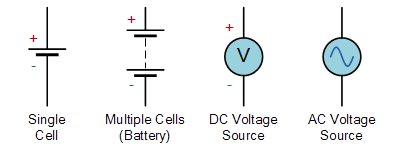
\includegraphics[width=7cm]{images/02}
	\caption{Voltage Symbols \citep{et-15}}
	\label{fig:voltage_symbols}
\end{figure}
%

\subsection*{Current}
Current, (SI Unit: $A$ - Ampere) is the movement or flow of electrical charge and is measured in Amperes. It is the continuous and uniform flow (called a drift) of electrons (the negative particles of an atom) around a circuit that are being pushed by the voltage source~\citep{et-15}.

%
\begin{figure}[ht]
	\centering
	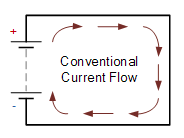
\includegraphics[width=4cm]{images/03}
	\caption{Current Symbols \citep{et-15}}
	\label{fig:current_symbols}
\end{figure}
%

\newpage
\subsection*{Resistance}
Resistance, (SI Unit: $\Omega$ - Ohms) of a circuit is its ability to resist or prevent the flow of current (electron flow) through itself making it necessary to apply a greater voltage to the electrical circuit to cause the current to flow again. Note that Resistance cannot be negative in value only positive~\citep{et-15}.

%
\begin{figure}[ht]
	\centering
	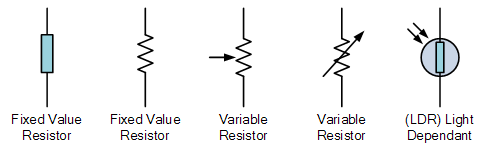
\includegraphics[width=8cm]{images/04}
	\caption{Resistance Symbols \citep{et-15}}
	\label{fig:resistance_symbols}
\end{figure}
%

\subsection*{Ohm's Law}
The following equation Ohm's Law explains the relationship between Voltage, Current and Resistance for an electrical circuit.

%
\begin{figure}[ht]
	\centering
	\begin{equation}
	V = I \times R
	\end{equation}
	\begin{equation}
	I = \frac{V}{R}
	\end{equation}
	\begin{equation}
	R = \frac{V}{I} 
	\end{equation}
	\caption{Ohm's Law}
	\label{fig:ohms_law_equation}
\end{figure}
%


\subsection*{Analogue vs Digital Signals}

The world we live in is an analogue one. There are an infinite number of possible combinations of colours smells and sounds. The digital world however is not infinite. It is discrete and finite where we are limited by several factors, such as memory and computational capabilities. In order to represent a real world thing digitally, it is by necessity that some information is lost.

\begin{description}
	\item[Analogue Signal Examples] \hfill \\
	The following are some examples of analogue signals:
	\begin{itemize}
		\item Temperature
		\item Sound
		\item EM Radiation
	\end{itemize}
	%
	\begin{figure}[ht]
		\centering
		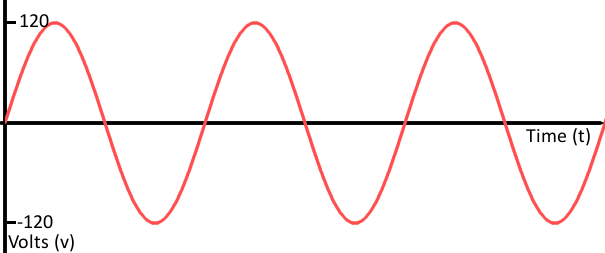
\includegraphics[width=8cm]{images/05}
		\caption{Analogue Signal \citep{sparkfun-15}}
		\label{fig:analogue_signal}
	\end{figure}
	%
	
	\item[Digital Signal Examples] \hfill \\
	The following are some examples of digital signals:
	\begin{itemize}
		\item Morse Code
		\item WIFI
		\item Binary
	\end{itemize}
	%
	\begin{figure}[ht]
		\centering
		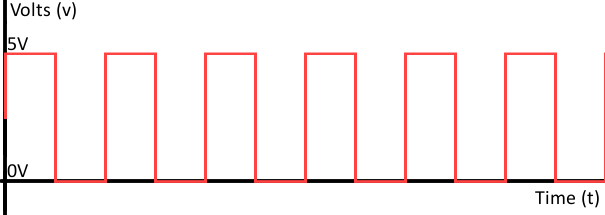
\includegraphics[width=8cm]{images/06}
		\caption{Digital Signal \citep{sparkfun-15}}
		\label{fig:digital_signal}
	\end{figure}
	%
\end{description}






\newpage
\section*{Basic Arduino Coding Concepts}
\addcontentsline{toc}{section}{Basic Arduino Coding Concepts}


\begin{description}
	\item[Variables] \hfill \\
	A variable is a way of naming and storing a value for later use by the program, such as data from a sensor or an intermediate value used in a calculation~\citep{arduino-15-b}.
	%
	\begin{table}
		\centering
		\begin{tabular}{p{4cm} l}
			\toprule
			Type & Example\\ \midrule
			char & 'a' \\
			string & 'Hello there' \\
			byte & 0 to 255 \\
			int & -32,768 to 32,767 \\
			unsigned int & 0 to 65,535 \\
			long & -2,147,483,648 to 2,147,483,647 \\
			unsigned long & 0 to 4,294,967,295 \\
			float & -3.4028235E38 to 3.4028235E38 \\
			\bottomrule
		\end{tabular}
		\caption{Variable Types in Wiring}
		\label{tab:wiring_variable_types}
	\end{table}
	%
	There are other more advanced data types such as Arrays, Strings and Pointers, which we won't be going into in this introduction. More information can be found regarding these data types online. See the Arduino online reference library at: https://www.arduino.cc/en/Reference/HomePage.
	
	\item[setup() function] \hfill \\
	The setup() function is called when a sketch starts. Use it to initialize variables, pin modes, start using libraries, etc. The setup function will only run once, after each powerup or reset of the Arduino board~\citep{arduino-15-c}.
	%
	\begin{lstlisting}
// setup initializes serial and the button pin
void setup()
{
  Serial.begin(9600);
}

// write to serial, then wait 2 seconds
void loop(){
  Serial.write("Hello World");
  delay(2000);
}
	\end{lstlisting}
	%

\newpage	
	\item[loop() function] \hfill \\
	After creating a setup() function, which initializes and sets the initial values, the loop() function does precisely what its name suggests, and loops consecutively, allowing your program to change and respond. Use it to actively control the Arduino board~\citep{arduino-15-d}.
	%
	\begin{lstlisting}
// Create int variable to represent
// a physical pin on the Arduino
int buttonPin = 3;

// setup initializes serial and the button pin
void setup()
{
  Serial.begin(9600);
  pinMode(buttonPin, INPUT);
}

// loop checks the button pin each time,
// and will send serial if it is pressed
void loop()
{
  if (digitalRead(buttonPin) == HIGH)
    Serial.write('H');
  else
    Serial.write('L');
  
  delay(1000);
}
	\end{lstlisting}
	%	
\end{description}
